\chapter{动态规划方法}\label{ch:dp}

\intro{``Those who cannot remember the past are condemned to repeat it.''\par
\hfill --- George Santayana\par
\hfill (但在动态规划中，我们恰恰利用``记住过去''来避免重复计算)\par
动态规划（Dynamic Programming，DP）是求解已知模型（complete knowledge）的MDP最优策略的一类经典方法。DP虽然不是现代大规模RL问题的直接解决方案（受限于维度灾难），但它是理解所有RL方法的理论基础。几乎所有的RL算法都可以看作是在模型未知时对DP思路的某种近似——策略评估近似、贪心策略改进近似，或两者的组合。}

% ======================================================================
\section{引言：DP在RL中的地位}
% ======================================================================

在深入具体算法之前，有必要先明确DP的使用前提和在RL大厦中的位置：

\textbf{DP的假设}（强假设——需要完整模型）：
\begin{enumerate}
    \item 状态集 $\states$ 和动作集 $\actions$ 是已知和有限的。
    \item 转移概率 $p(s', r \mid s, a)$ 对所有的 $(s, a, s', r)$ 都是已知的。
    \item 奖励函数是已知的。
\end{enumerate}

在这些假设下，DP能够精确求解MDP。实际上，DP的核心思想——利用值函数的递归结构（Bellman方程）将大问题分解为子问题——是所有RL方法的共同基因。

\textbf{DP的关键局限}：
\begin{itemize}
    \item \textbf{维度灾难 (Curse of Dimensionality)}：状态数 $|\states|$ 随状态变量的数量指数增长。一个 $d$ 维网格、每维 $k$ 个格点的状态空间大小为 $k^d$。对于 $d=10, k=100$，$|\states| = 100^{10} = 10^{20}$——在宇宙年龄尺度下也无法遍历。
    \item \textbf{需要完整模型}：多数现实问题中，环境模型 $p(s', r \mid s, a)$ 是未知的。
\end{itemize}

尽管有这些局限，DP为后续章节的模型自由方法提供了：
\begin{itemize}
    \item 收敛性的理论基准（对渐进性能的上限）
    \item 算法设计的结构性框架（评估/改进交替的GPI模式）
    \item 启发式思想（bootstrap、异步更新、优先扫描等）
\end{itemize}

% ======================================================================
\section{策略评估 (Policy Evaluation)}
% ======================================================================

% ----------------------------------------------------------------------
\subsection{问题陈述}
% ----------------------------------------------------------------------

\textbf{策略评估}（也称\textbf{预测问题}）：给定一个MDP和策略 $\pi$，计算该策略下的状态值函数 $V^{\pi}(s)$，对所有 $s \in \states$。

如果MDP规模很小（$|\states| \sim 10^3$），可以使用第\ref{ch:mdp}章导出的解析解：
\[
\mathbf{V}^{\pi} = (\mathbf{I} - \gamma \mathbf{P}^{\pi})^{-1} \mathbf{R}^{\pi}
\]
但这需要 $O(|\states|^3)$ 的计算量和 $O(|\states|^2)$ 的存储，对稍大规模的问题即变得不可行。

% ----------------------------------------------------------------------
\subsection{迭代策略评估}
% ----------------------------------------------------------------------

\textbf{核心思想}：将Bellman期望方程转化为迭代更新规则。

从任意初始值函数 $V_0$（例如全零向量）出发，迭代施加Bellman期望算子：
\[
V_{k+1}(s) \leftarrow \sum_{a} \pi(a \mid s) \sum_{s', r} p(s', r \mid s, a) \left[ r + \gamma V_k(s') \right]
\]
对所有的 $s \in \states$。当 $k \to \infty$ 时，序列 $\{V_k\}$ 收敛于 $V^{\pi}$。

\begin{myalgorithm}{迭代策略评估}
\begin{enumerate}
    \item \textbf{输入}：待评估的策略 $\pi$，收敛阈值 $\theta > 0$（小正数）。
    \item \textbf{初始化}：$V(s) \leftarrow 0$ 对所有 $s \in \states$（终止状态除外，恒为 $0$）。
    \item \textbf{循环}：
    \begin{enumerate}
        \item $\Delta \leftarrow 0$
        \item 对每个 $s \in \states$（非终止状态）：
        \begin{enumerate}
            \item $v \leftarrow V(s)$
            \item $V(s) \leftarrow \sum_{a} \pi(a \mid s) \sum_{s', r} p(s', r \mid s, a) \left[ r + \gamma V(s') \right]$
            \item $\Delta \leftarrow \max(\Delta, |v - V(s)|)$
        \end{enumerate}
        \item 若 $\Delta < \theta$，停止并返回 $V \approx V^{\pi}$。
    \end{enumerate}
\end{enumerate}
\end{myalgorithm}

\textbf{停止准则的解读}：$\Delta = \max_s |V_{k+1}(s) - V_k(s)|$ 是值函数迭代两步之间的最大变化量。当 $\Delta < \theta$ 时，可认为值函数已``足够接近''真实 $V^{\pi}$。基于Banach不动点定理的后验估计：
\[
\|V_k - V^{\pi}\|_\infty \le \frac{\gamma}{1 - \gamma} \|V_k - V_{k-1}\|_\infty \le \frac{\gamma}{1 - \gamma} \theta
\]
故 $\Delta < \theta$ 保证了解与真值的 $L_\infty$ 距离不超过 $\frac{\gamma}{1-\gamma} \theta$。

% ----------------------------------------------------------------------
\subsection{收敛性分析}
% ----------------------------------------------------------------------

\begin{myTheorem}{迭代策略评估的收敛性}
设 $V_0$ 为任意初始值函数。由迭代 $V_{k+1} = \mathcal{T}^{\pi} V_k$ 生成的序列 $\{V_k\}$ 以速率 $\gamma^k$ 收敛到唯一不动点 $V^{\pi}$：
\[
\|V_k - V^{\pi}\|_\infty \le \gamma^k \|V_0 - V^{\pi}\|_\infty
\]
\end{myTheorem}

\begin{proof}
这是Banach不动点定理的直接推论。第\ref{ch:mdp}章已证明 $\mathcal{T}^{\pi}$ 在 $L_\infty$ 范数下是以 $\gamma$ 为压缩因子的压缩映射：
\[
\|\mathcal{T}^{\pi} V_1 - \mathcal{T}^{\pi} V_2\|_\infty \le \gamma \|V_1 - V_2\|_\infty
\]
对 $V_k = \mathcal{T}^{\pi} V_{k-1} = (\mathcal{T}^{\pi})^k V_0$ 和 $V^{\pi} = \mathcal{T}^{\pi} V^{\pi}$：
\begin{align*}
\|V_k - V^{\pi}\|_\infty &= \|(\mathcal{T}^{\pi})^k V_0 - (\mathcal{T}^{\pi})^k V^{\pi}\|_\infty \\
&\le \gamma^k \|V_0 - V^{\pi}\|_\infty
\end{align*}
由于 $\gamma < 1$，$\gamma^k \to 0$，证毕。
\end{proof}

\textbf{收敛速率}：每次迭代使误差缩小 $\gamma$ 倍。若 $\gamma = 0.9$，每步误差减少 $10\%$——这意味着需要大约 $230$ 步才能将初始误差缩小到 $10^{-10}$ 倍（$0.9^{230} \approx 3 \times 10^{-11}$）。若 $\gamma = 0.99$，则需约 $2300$ 步。这就是为什么接近1的折扣因子会使DP收敛变慢。

% ----------------------------------------------------------------------
\subsection{GridWorld策略评估实例}
% ----------------------------------------------------------------------

回到第\ref{ch:mdp}章介绍的 $4 \times 4$ GridWorld。我们对均匀随机策略（每个动作概率 $0.25$）执行策略评估。$\gamma = 0.9$，非终止状态奖励为 $-1$（为简化演示取 $-1$ 而非 $-0.04$）。

\begin{center}
\begin{tikzpicture}[scale=1.3]
    \draw[step=1.0, gray, very thin] (0,0) grid (4,4);
    
    % V values after convergence (approximate)
    \node at (0.5, 3.5) {$0.0$};  % terminal +1
    \node at (1.5, 3.5) {$0.6$};
    \node at (2.5, 3.5) {$0.7$};
    \node at (3.5, 3.5) {$0.7$};
    \node at (0.5, 2.5) {$0.3$};
    \node at (1.5, 2.5) {$0.5$};
    \node at (2.5, 2.5) {$0.6$};
    \node at (3.5, 2.5) {$0.4$};
    \node at (0.5, 1.5) {$-0.1$};
    \node at (1.5, 1.5) {$0.1$};
    \node at (2.5, 1.5) {$0.0$};
    \node at (3.5, 1.5) {$-0.5$};
    \node at (0.5, 0.5) {$-1.1$};
    \node at (1.5, 0.5) {$-0.8$};
    \node at (2.5, 0.5) {$-0.8$};
    \node at (3.5, 0.5) {$0.0$};  % terminal -1
    
    \fill[red!15] (0,3) rectangle (1,4);
    \fill[red!15] (3,0) rectangle (4,1);
    \node[red] at (0.5, 4.3) {$R=+1$ (终止)};
    \node[red] at (3.5, -0.3) {$R=-1$ (终止)};
\end{tikzpicture}
\end{center}

\textbf{观察}：
\begin{itemize}
    \item 均匀随机策略下，值函数在正奖励终止状态附近为正（``好''的区域），在负奖励终止状态附近为负（``坏''的区域）。
    \item 远离终止状态的值接近 $0$：因为随机游走到达终点的概率较低，且每步 $-1$ 的惩罚被 $\gamma^k$ 折扣后累计不大。
    \item 某些状态的值呈非对称分布，反映了墙体的阻挡效应（撞墙反弹）。
\end{itemize}

\textbf{迭代过程}（前几步的 $V$ 变化）：
\begin{itemize}
    \item $k=0$：$V_0(s) = 0$ 对所有 $s$。
    \item $k=1$：$V_1(s) = -1$（所有非终止状态，因为每步获得 $-1$）。
    \item $k=2$：$V_2(s_2) \approx -1 + 0.9 \times 0.25 \times (+1) \approx -0.775$（开始感知到正奖励终点的影响）。
    \item $\dots$
    \item $k \approx 100$：已接近收敛值。
\end{itemize}

% ======================================================================
\section{策略改进 (Policy Improvement)}
% ======================================================================

策略评估回答了``给定 $\pi$，$V^{\pi}$ 是什么''。但我们的终极目标不是评价策略，而是\textbf{改进}策略。策略改进定理为这一目标提供了理论基础。

% ----------------------------------------------------------------------
\subsection{策略改进定理}
% ----------------------------------------------------------------------

\begin{myTheorem}{策略改进定理 (Policy Improvement Theorem)}
设 $\pi$ 和 $\pi'$ 为确定性策略。如果对所有 $s \in \states$：
\begin{myformula}
Q^{\pi}(s, \pi'(s)) \ge V^{\pi}(s)
\end{myformula}
则改进后的策略 $\pi'$ 至少和 $\pi$ 一样好：
\[
V^{\pi'}(s) \ge V^{\pi}(s), \quad \forall s \in \states
\]
若上式中对至少一个状态有严格大于，则 $\pi'$ 严格优于 $\pi$。
\end{myTheorem}

\begin{proof}
这个证明是RL中一个经典且优雅的论证。我们逐层展开。

\begin{align*}
V^{\pi}(s) &\le Q^{\pi}(s, \pi'(s)) \quad \text{(前提条件)} \\
&= \E[R_{t+1} + \gamma V^{\pi}(S_{t+1}) \mid S_t = s, A_t = \pi'(s)] \\
&\le \E[R_{t+1} + \gamma Q^{\pi}(S_{t+1}, \pi'(S_{t+1})) \mid S_t = s, A_t = \pi'(s)] \quad \text{(再次使用前提条件)} \\
&= \E_{\pi'}[R_{t+1} + \gamma \E[R_{t+2} + \gamma V^{\pi}(S_{t+2}) \mid S_{t+1}, A_{t+1} = \pi'(S_{t+1})] \mid S_t = s] \\
&\le \dots \quad \text{(反复展开)}
\end{align*}

不断将 $V^{\pi}$ 替换为 $Q^{\pi}(\cdot, \pi'(\cdot))$，最终得到：
\begin{align*}
V^{\pi}(s) &\le \E_{\pi'}[R_{t+1} + \gamma R_{t+2} + \gamma^2 R_{t+3} + \dots \mid S_t = s] \\
&= V^{\pi'}(s)
\end{align*}
\end{proof}

\textbf{定理的直观含义}：如果你在每个状态下选一个比起当前策略更好的动作（以 $Q^{\pi}$ 为准），然后一直执行这个新策略，那么新策略整体上至少不会比原策略差。

% ----------------------------------------------------------------------
\subsection{贪心策略改进}
% ----------------------------------------------------------------------

基于策略改进定理，一种自然的策略改进方法是\textbf{贪心策略}：对每个状态，选择最大化 $Q^{\pi}(s, a)$ 的动作：
\begin{myformula}
\pi'(s) = \arg\max_{a \in \actions} Q^{\pi}(s, a) = \arg\max_{a \in \actions} \sum_{s', r} p(s', r \mid s, a) \left[ r + \gamma V^{\pi}(s') \right]
\end{myformula}

若有多个最大化动作，可以任意选择其中之一（或任意概率分配）。这种改进方式产生的新策略满足 $Q^{\pi}(s, \pi'(s)) = \max_a Q^{\pi}(s, a) \ge \sum_a \pi(a \mid s) Q^{\pi}(s, a) = V^{\pi}(s)$，因此满足策略改进定理的条件，必然是改进（或至少不退化）。

\begin{remark}
\textbf{策略改进何时终止？} 当贪心策略不再改变时，即对所有 $s$：
\[
\pi(s) = \arg\max_a Q^{\pi}(s, a)
\]
此时 $\pi$ 满足 Bellman 最优方程，因此 $\pi = \pi^{*}$。直观上：如果按照当前的 $\pi$ 评估出的 $V^{\pi}$ 的贪心策略就是 $\pi$ 本身，那 $\pi$ 已经是最优的了（已无改进空间）。
\end{remark}

\begin{example}
\textbf{GridWorld策略改进演示}。在第\ref{ch:mdp}章的GridWorld上，对均匀随机策略执行一轮评估后，在各状态按贪心动作改进策略。

对状态 $s_2$（位置 (2, 4)），四个动作的 $Q$ 值（近似）为：
\begin{itemize}
    \item 北：碰墙，大致 $Q \approx -1 + 0.9 V(s_2) \approx -1 + 0.9 \times 0.6 = -0.46$
    \item 南：$Q \approx -1 + 0.9 V(s_6) \approx -1 + 0.9 \times 0.5 = -0.55$
    \item 东：$Q \approx -1 + 0.9 V(s_3) \approx -1 + 0.9 \times 0.0 = -1.0$（直接进入+1终止态，但$V(s_3)=0$因为是终止态）
    \item \textbf{西}：$Q \approx -1 + 0.9 V(s_1) \approx -1 + 0.9 \times 0.6 = -0.46$
\end{itemize}
（注意：这里的数值是示意性的，实际Q值因有转移随机性而不同。准确说，东移有较高概率进入正奖励终止态，$Q$值应最高。）

改进后的策略会选择最优动作。在大多数靠近正奖励的状态，最优动作指向正奖励终点方向；靠近负奖励终点的状态则远离它。
\end{example}

% ======================================================================
\section{策略迭代 (Policy Iteration)}
% ======================================================================

% ----------------------------------------------------------------------
\subsection{算法描述}
% ----------------------------------------------------------------------

策略迭代将策略评估和策略改进交替进行，形成一个收敛到最优策略的递归循环：

\begin{center}
\begin{tikzpicture}[node distance=2cm]
    \node[draw, rounded corners, fill=blue!15, minimum width=3.5cm, minimum height=1.2cm] (eval) {\textbf{策略评估}};
    \node[draw, rounded corners, fill=green!15, minimum width=3.5cm, minimum height=1.2cm, right=0.5cm of eval] (improve) {\textbf{策略改进}};
    
    \draw[->, thick] (eval.east) -- node[above] {$V^{\pi}$} (improve.west);
    \draw[->, thick, bend right=40] (improve.south) to node[below] {$\pi \leftarrow \pi'$（贪心）} (eval.south);
    
    \node[below=0.5cm of eval] (pi) {$\pi \xrightarrow{E} V^{\pi}$};
    \node[below=0.5cm of improve] (pi2) {$V^{\pi} \xrightarrow{I} \pi'$};
    
    \node[draw, rounded corners, fill=gray!10, minimum width=9cm, minimum height=0.6cm, above=2.5cm of eval] (title) {\textbf{策略迭代循环：} $\pi_0 \xrightarrow{E} V^{\pi_0} \xrightarrow{I} \pi_1 \xrightarrow{E} V^{\pi_1} \xrightarrow{I} \pi_2 \xrightarrow{E} \dots \xrightarrow{I} \pi^{*}$};
\end{tikzpicture}
\end{center}

\begin{myalgorithm}{策略迭代 (Policy Iteration)}
\begin{enumerate}
    \item \textbf{初始化}：
    \begin{itemize}
        \item $V(s) \in \R$ 对所有 $s \in \states$ 任意初始化。
        \item $\pi(s) \in \actions(s)$ 对所有 $s \in \states$ 任意初始化（例如均匀随机）。
    \end{itemize}
    \item \textbf{策略评估 (Policy Evaluation)}：
    \begin{enumerate}
        \item 循环直到收敛（$\Delta < \theta$）：
        \[
        V(s) \leftarrow \sum_{s', r} p(s', r \mid s, \pi(s)) \left[ r + \gamma V(s') \right]
        \]
        （对确定性 $\pi$，$\pi(a \mid s)$ 退化为极端分布）
    \end{enumerate}
    \item \textbf{策略改进 (Policy Improvement)}：
    \begin{enumerate}
        \item $\mathrm{policy\_stable} \leftarrow \mathrm{true}$
        \item 对每个 $s \in \states$：
        \begin{enumerate}
            \item $\text{old\_action} \leftarrow \pi(s)$
            \item $\pi(s) \leftarrow \arg\max_{a} \sum_{s', r} p(s', r \mid s, a) \left[ r + \gamma V(s') \right]$
            \item 若 $\text{old\_action} \neq \pi(s)$，则 $\mathrm{policy\_stable} \leftarrow \mathrm{false}$
        \end{enumerate}
        \item 若 $\mathrm{policy\_stable}$，停止并返回 $V$ 和 $\pi$（即 $V^{*}$ 和 $\pi^{*}$）。
        \item 否则，转步骤2。
    \end{enumerate}
\end{enumerate}
\end{myalgorithm}

% ----------------------------------------------------------------------
\subsection{收敛性与复杂度}
% ----------------------------------------------------------------------

\begin{myTheorem}{策略迭代的收敛性}
在有限MDP上，策略迭代在有限步内收敛到最优策略 $\pi^{*}$ 和最优值函数 $V^{*}$。
\end{myTheorem}

\begin{proof}
有限MDP的策略空间是有限的：确定性策略总数为 $|\actions|^{|\states|}$（每个状态选择 $|\actions|$ 个动作之一）。每一次策略改进都严格优于前一个策略（除非已是最优），因此不会重复同一个非最优策略。由于策略数为有限，算法必然在有限步内终止于最优策略。
\end{proof}

\textbf{每次策略评估的计算量}：每次扫描所有 $|\states|$ 个状态，每个状态需要遍历 $|\actions|$ 个动作和 $|\states|$ 个后继状态，复杂度为 $O(|\states|^2 |\actions|)$。策略评估需要 $\approx \frac{\log(1/\varepsilon)}{1-\gamma}$ 次扫描（取决于 $\gamma$ 和精度 $\varepsilon$）。

\textbf{策略改进的复杂度}：$O(|\states|^2 |\actions|)$（与一次评估扫描相同）。

\textbf{策略迭代的次数}：尽管理论上最多 $|\actions|^{|\states|}$ 次迭代，实际上通常只需很少的迭代次数（典型为 5~20 次）即可收敛。

% ----------------------------------------------------------------------
\subsection{GridWorld策略迭代实例}
% ----------------------------------------------------------------------

对 $4 \times 4$ GridWorld，$\gamma = 0.9$，应用策略迭代：

\begin{center}
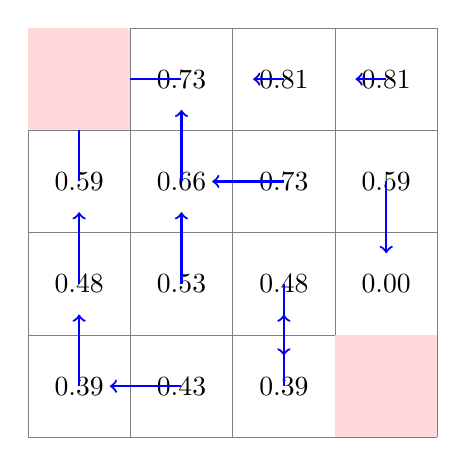
\begin{tikzpicture}[scale=1.3]
    \draw[step=1.0, gray, very thin] (0,0) grid (4,4);
    
    % Optimal V values (approximate)
    \node at (0.5, 3.5) {$0.00$};
    \node at (1.5, 3.5) {$0.73$};
    \node at (2.5, 3.5) {$0.81$};
    \node at (3.5, 3.5) {$0.81$};
    \node at (0.5, 2.5) {$0.59$};
    \node at (1.5, 2.5) {$0.66$};
    \node at (2.5, 2.5) {$0.73$};
    \node at (3.5, 2.5) {$0.59$};
    \node at (0.5, 1.5) {$0.48$};
    \node at (1.5, 1.5) {$0.53$};
    \node at (2.5, 1.5) {$0.48$};
    \node at (3.5, 1.5) {$0.00$};
    \node at (0.5, 0.5) {$0.39$};
    \node at (1.5, 0.5) {$0.43$};
    \node at (2.5, 0.5) {$0.39$};
    \node at (3.5, 0.5) {$0.00$};
    
    % Optimal policy arrows
    \draw[->, blue, thick] (1.5,3.5) -- (0.8,3.5);
    \draw[->, blue, thick] (2.5,3.5) -- (2.2,3.5);
    \draw[->, blue, thick] (3.5,3.5) -- (3.2,3.5);
    \draw[->, blue, thick] (0.5,2.5) -- (0.5,3.2);
    \draw[->, blue, thick] (1.5,2.5) -- (1.5,3.2);
    \draw[->, blue, thick] (2.5,2.5) -- (1.8,2.5);
    \draw[->, blue, thick] (3.5,2.5) -- (3.5,1.8);
    \draw[->, blue, thick] (0.5,1.5) -- (0.5,2.2);
    \draw[->, blue, thick] (1.5,1.5) -- (1.5,2.2);
    \draw[->, blue, thick] (2.5,1.5) -- (2.5,0.8);
    \draw[->, blue, thick] (0.5,0.5) -- (0.5,1.2);
    \draw[->, blue, thick] (1.5,0.5) -- (0.8,0.5);
    \draw[->, blue, thick] (2.5,0.5) -- (2.5,1.2);
    
    \fill[red!15] (0,3) rectangle (1,4);
    \fill[red!15] (3,0) rectangle (4,1);
\end{tikzpicture}
\end{center}

\textbf{关键观察}：
\begin{itemize}
    \item 最优策略将所有状态导向 $+1$ 奖励的终点。
    \item 最优值函数从 $+1$ 终点向外递减，衰减因子即为 $0.9$ 递减。
    \item $s_9$（位置 (2,1)，即最右下角非终止态）和 $s_{13}$（位置 (1,0)）有一个有趣的``远离 $-1$''的趋势，但由于值迭代会寻找整体最优，它们也可能被拖向 $+1$（取决于具体奖励设置）。
    \item 与均匀随机策略的值函数相比，最优值函数显著更高——这正是``好决策''的回报。
\end{itemize}

% ======================================================================
\section{值迭代 (Value Iteration)}
% ======================================================================

策略迭代的瓶颈在于每次外循环需要完整的策略评估（多轮内循环扫描直至收敛）。值迭代优雅地将评估和改进``合二为一''，用一次扫描兼做评估和改进。

% ----------------------------------------------------------------------
\subsection{算法推导}
% ----------------------------------------------------------------------

\textbf{思想}：如果我们在策略评估中只执行\textbf{一次}扫描（而非多次直到收敛），然后立即进行策略改进，会发生什么？将两者浓缩为一步更新：
\[
V_{k+1}(s) \leftarrow \max_{a \in \actions} \sum_{s', r} p(s', r \mid s, a) \left[ r + \gamma V_k(s') \right]
\]

这就是\textbf{值迭代}！它将Bellman最优方程直接转化为迭代更新规则。初看起来，这是把策略改进的 $\max_a$ 操作嵌入到了评估扫描中。实际上，这是在迭代求解Bellman最优算子 $\mathcal{T}^{*}$ 的不动点：
\[
V_{k+1} = \mathcal{T}^{*} V_k, \quad \text{其中 } (\mathcal{T}^{*} V)(s) = \max_a \sum_{s', r} p(s', r \mid s, a) [r + \gamma V(s')]
\]

\begin{myalgorithm}{值迭代 (Value Iteration)}
\begin{enumerate}
    \item \textbf{初始化}：$V(s) \leftarrow 0$ 对所有 $s \in \states$（终止状态为 $0$）。
    \item \textbf{循环}：
    \begin{enumerate}
        \item $\Delta \leftarrow 0$
        \item 对每个 $s \in \states$：
        \begin{enumerate}
            \item $v \leftarrow V(s)$
            \item $V(s) \leftarrow \max_{a} \sum_{s', r} p(s', r \mid s, a) \left[ r + \gamma V(s') \right]$
            \item $\Delta \leftarrow \max(\Delta, |v - V(s)|)$
        \end{enumerate}
        \item 若 $\Delta < \theta$，停止迭代。
    \end{enumerate}
    \item \textbf{提取最优策略}：
    \[
    \pi(s) \leftarrow \arg\max_{a} \sum_{s', r} p(s', r \mid s, a) \left[ r + \gamma V(s') \right]
    \]
    对所有 $s \in \states$。
\end{enumerate}
\end{myalgorithm}

% ----------------------------------------------------------------------
\subsection{收敛性讨论}
% ----------------------------------------------------------------------

\begin{myTheorem}{值迭代的收敛性}
Bellman最优算子 $\mathcal{T}^{*}$ 在 $L_\infty$ 范数下也是以 $\gamma$ 为压缩因子的压缩映射。因此值迭代 $V_{k+1} = \mathcal{T}^{*} V_k$ 对任意初始 $V_0$ 收敛到 $V^{*}$：
\[
\|V_k - V^{*}\|_\infty \le \gamma^k \|V_0 - V^{*}\|_\infty
\]
\end{myTheorem}

\begin{proof}
对任意 $V_1, V_2$：
\begin{align*}
\| \mathcal{T}^{*} V_1 - \mathcal{T}^{*} V_2 \|_\infty &= \max_s \left| \max_a \sum_{s', r} p(s', r \mid s, a) [r + \gamma V_1(s')] - \max_a \sum_{s', r} p(s', r \mid s, a) [r + \gamma V_2(s')] \right|
\end{align*}

利用不等式 $|\max_a f(a) - \max_a g(a)| \le \max_a |f(a) - g(a)|$：
\begin{align*}
&\le \max_s \max_a \left| \sum_{s', r} p(s', r \mid s, a) \cdot \gamma [V_1(s') - V_2(s')] \right| \\
&\le \max_s \max_a \gamma \sum_{s'} p(s' \mid s, a) |V_1(s') - V_2(s')| \\
&\le \gamma \max_{s'} |V_1(s') - V_2(s')| = \gamma \|V_1 - V_2\|_\infty
\end{align*}
由Banach不动点定理，序列收敛到唯一不动点 $V^{*}$（Bellman最优方程的解）。
\end{proof}

\textbf{与策略迭代的关系}：值迭代可视为策略迭代的一种极端形式——在每次策略评估中只做一次扫描（$k=1$ 轮内循环）。虽然每次外循环的评估不精确，但通过大量外循环的迭代，最终仍收敛到最优值函数。

% ----------------------------------------------------------------------
\subsection{从 $V^{*}$ 提取 $\pi^{*}$}
% ----------------------------------------------------------------------

值迭代直接求得 $V^{*}$ 而非 $\pi^{*}$。从 $V^{*}$ 恢复最优策略只需一次贪心选择：
\[
\pi^{*}(s) = \arg\max_{a} \sum_{s', r} p(s', r \mid s, a) [r + \gamma V^{*}(s')]
\]

一个微妙的点是：可能存在多个动作同时最大化Q值（例如有两条等价的最优路径）。此时任意选择其中之一都是最优的。但在值迭代的中间阶段（$V_k$ 尚未收敛到 $V^{*}$），$V_k$ 对应的贪心策略不一定是最终的 $\pi^{*}$——贪心策略可能比 $V_k$ 本身更早稳定。这意味着：即使 $V_k$ 还不够精确，其贪心策略可能已经是最优的了。

\begin{remark}
\textbf{贪心策略早于值函数收敛}：在许多问题中，当值迭代只运行到 ``$V_k$ 的贪心策略不再变化'' 时即可停止（即使 $\Delta$ 刚下降了几个数量级），因为此时最优策略已经找到，继续迭代只是在精细调优值函数的绝对值。这可以在实践中节约大量计算。
\end{remark}

% ----------------------------------------------------------------------
\subsection{策略迭代 vs 值迭代}
% ----------------------------------------------------------------------

\begin{center}
\begin{tabular}{p{5cm} p{5cm}}
\hline
\textbf{策略迭代} & \textbf{值迭代} \\
\hline
每外循环：完整策略评估（多轮扫描至收敛） & 每扫描：一次更新，评估+改进合一 \\
内循环扫描多（收敛慢于外循环） & 只有外层循环，每次扫描简单 \\
总扫描次数较少（外循环次数 $\approx 5\sim20$） & 总扫描次数较多（需 $\sim 100+$） \\
每次扫描计算量大（全评估） & 每次扫描计算量小（单步更新） \\
对 $\gamma$ 接近 $1$ 更敏感 & $\gamma$ 影响的是全扫描次数 \\
\hline
\end{tabular}
\end{center}

实践中通常使用值迭代，因为它实现更简单且总效率往往不差。对于特别大的状态空间，策略评估的完整收敛成本过高，值迭代的一步评估思路更实际。

% ======================================================================
\section{广义策略迭代 (Generalized Policy Iteration, GPI)}
% ======================================================================

\begin{mydefinition}{广义策略迭代}
GPI是指\textbf{几乎所有RL方法}的共同框架：策略评估和策略改进这两个过程交替或交织进行，互相促进，最终驱动策略和值函数同时趋近最优。
\end{mydefinition}

\begin{center}
\begin{tikzpicture}[scale=1.2]
    % Axes
    \draw[->] (0,0) -- (6,0) node[right] {$\pi$ 是最优的？};
    \draw[->] (0,0) -- (0,5) node[above] {$V$ 能准确评估 $\pi$？};
    
    % Policy improvement arrow
    \draw[->, red, very thick, bend left=60] (0.5,5.2) to node[above] {\textbf{策略改进}} (5.5,0.2);
    \draw[->, red, very thick] (4.5,-0.3) to (5.5,0.2);
    
    % S-shaped trajectory
    \draw[blue, thick] (1.0,0.5) -- (1.8,3.5);
    \draw[blue, thick] (1.8,3.5) -- (2.5,2.0) -- (3.5,4.5) -- (4.5,3.5) -- (5.0,5.0);
    \fill[blue] (5.0,5.0) circle (2pt) node[above right] {$(\pi^{*}, V^{*})$};
    
    % Annotations
    \node[below=0.3cm] at (3,0) {\small 策略改进使策略更接近最优};
    \node[left=0.3cm, rotate=90] at (0,2.5) {\small 策略评估使值函数更精确};
    
    % Legend
    \node[red] at (3, -0.8) {$\longrightarrow$ 策略改进方向};
    \node[blue] at (3, -1.2) {$\longrightarrow$ GPI轨迹};
\end{tikzpicture}
\end{center}

\textbf{GPI的精髓}：
\begin{itemize}
    \item \textbf{评估与改进相互对抗}：评估将值函数拉向当前策略的真实值；改进将策略拉离当前策略（朝向贪心方向）。两者形成``推-拉''动态。
    \item \textbf{两者最终和解于最优}：当且仅当策略对自身的值函数贪心时，评估和改进达成一致——此时策略即为最优。
    \item \textbf{几乎任何顺序均可}：可以在每次评估扫描后改进，可以评估若干扫描后改进一次，可以只改进部分状态……只要两个过程都持续进行，且没有过程完全停止（除非已达最优），GPI最终收敛到最优解。
\end{itemize}

\begin{myTheorem}{GPI的收敛性（非正式）}
在一个有限MDP中，只要策略评估和策略改进过程无限次地对每个状态执行，且评估最终准确地识别当前策略的值函数，GPI必然收敛到最优策略和最优值函数。
\end{myTheorem}

\textbf{GPI是RL的统一范式}：
\begin{itemize}
    \item \textbf{动态规划}：精确模型下的精确评估+精确改进。
    \item \textbf{Monte Carlo}：采样下的近似评估+$\epsilon$-贪心改进。
    \item \textbf{TD学习}：bootstrap近似评估+$\epsilon$-贪心改进。
    \item \textbf{Actor-Critic}：Actor（策略改进）和Critic（策略评估）两个显式组件。
    \item \textbf{DQN}：Q-learning（值迭代的采样版本）= GPI，但评估和改进合并在单步更新中。
\end{itemize}

% ======================================================================
\section{异步动态规划}
% ======================================================================

前述DP方法都是\textbf{同步}的——每步扫描更新\textbf{所有}状态后才进入下一步。这对大规模状态空间（$|\states| > 10^6$）是不可承受的。异步DP放松了这一约束，允许以任意顺序更新状态。

% ----------------------------------------------------------------------
\subsection{就地动态规划 (In-Place DP)}
% ----------------------------------------------------------------------

\textbf{同步DP}：
\begin{align*}
V_{k+1}(s) &\leftarrow \sum_a \pi(a \mid s) \sum_{s', r} p(s', r \mid s, a) [r + \gamma V_k(s')], \quad \forall s
\end{align*}
同步DP需要同时保留新旧两个数组，内存为 $2 \cdot |\states|$。

\textbf{就地DP}：只维护一个值函数数组，使用最新的值：
\[
V(s) \leftarrow \sum_a \pi(a \mid s) \sum_{s', r} p(s', r \mid s, a) [r + \gamma V(s')]
\]
更新 $V(s_1)$ 后立即使用新的 $V(s_1)$ 来更新 $V(s_2)$（如果 $s_2$ 的更新依赖 $s_1$）。这类似于Gauss-Seidel迭代法（相比Jacobi迭代的同步版本）。

\textbf{就地DP的优势}：
\begin{itemize}
    \item 内存减半（$|\states|$ 而非 $2|\states|$）。
    \item 通常收敛更快，因为新信息立即被后续更新利用。
    \item 更新顺序可以影响收敛速度——状态按某种``重要性''顺序更新可能显著加速。
\end{itemize}

% ----------------------------------------------------------------------
\subsection{优先扫描 (Prioritized Sweeping)}
% ----------------------------------------------------------------------

并非所有状态的价值相同——某些状态的值函数变化剧烈（如靠近奖励源），某些则几乎不变。优先扫描将计算资源集中在``最需要更新''的状态上。

\begin{myalgorithm}{优先扫描 (Prioritized Sweeping)}
\begin{enumerate}
    \item 维护一个优先队列，键为状态的Bellman更新量（预期变化量）。
    \item 初始化：对所有状态计算Bellman误差，插入优先队列。
    \item \textbf{循环}直到收敛或预算耗尽：
    \begin{enumerate}
        \item 从优先队列取出优先级最高的状态 $s$。
        \item 仅对 $s$ 执行Bellman更新：$V(s) \leftarrow \max_a \sum_{s', r} p(s', r \mid s, a) [r + \gamma V(s')]$。
        \item 计算 $s$ 的值变化量 $\delta = |V_{\text{new}}(s) - V_{\text{old}}(s)|$。
        \item 对所有可能转移到 $s$ 的前驱状态 $\bar{s}$（满足 $p(s \mid \bar{s}, a) > 0$ 的 $\bar{s}$），将其优先级提升（加上 $\gamma \cdot p(s \mid \bar{s}, a) \cdot \delta$ 相关的量）。
    \end{enumerate}
\end{enumerate}
\end{myalgorithm}

\textbf{思想}：当状态 $s$ 的值发生变化时，所有能到达 $s$ 的前驱状态的值也会受到影响（通过Bellman方程的递归）。这个影响以 $\gamma$ 为折扣传播。优先扫描正是沿着反向转移图传播更新优先级。

\textbf{效果}：在稀疏奖励的环境中（如迷宫寻路，仅在终点有奖励），优先扫描从终点反向向外广播值更新，比同步扫描（每次更新所有状态）高效得多。经验表明，优先扫描常能将收敛所需的总更新次数减少 $1\sim2$ 个数量级。

% ----------------------------------------------------------------------
\subsection{实时动态规划 (Real-Time DP, RTDP)}
% ----------------------------------------------------------------------

RTDP是一种\textbf{在线、基于轨迹}的异步DP变体。智能体在与环境（或模拟器）交互的过程中，仅更新实际访问到的状态的值函数。

\textbf{RTDP的更新规则}（对访问到的状态 $S_t$）：
\[
V(S_t) \leftarrow \max_a \sum_{s', r} p(s', r \mid S_t, a) [r + \gamma V(s')]
\]
随后智能体按当前贪心策略选择动作并转移到下一状态。

\textbf{RTDP的优势}：
\begin{itemize}
    \item \textbf{聚焦相关性}：只更新可能被最优策略访问到的状态（``相关状态''），忽略不相关的状态空间区域。对于大状态空间、稀疏奖励的问题，这可以极大节约计算。
    \item \textbf{在线与离线结合}：可在仿真环境中运行RTDP以学习（或改进）策略，然后部署到真实环境。
    \item \textbf{随时终止性}：即使未完全收敛，RTDP的当前贪心策略在已探索的``相关状态''区域通常是准最优的。
\end{itemize}

\textbf{RTDP的收敛性}：在适当的探索条件下（所有相关状态被无限次访问），RTDP收敛到最优值函数。相关状态集合由最优策略可到达的状态定义。

RTDP可以看作值迭代的采样异步版本，也可以视为Q-learning在已知模型条件下的原型。两者都在实际访问到的状态上做Bellman更新，区别在于Q-learning不需要环境模型（用 $r + \gamma \max_{a'} Q(s', a')$ 取代求期望），而RTDP需要模型来精确计算后继状态的期望。

% ======================================================================
\section{DP的效率与局限}
% ======================================================================

% ----------------------------------------------------------------------
\subsection{计算复杂度分析}
% ----------------------------------------------------------------------

设 $n = |\states|$，$m = |\actions|$。

\begin{itemize}
    \item \textbf{策略评估（一次扫描）}：$O(n^2 m)$。对每个 $s$（$n$个），遍历每个 $a$（$m$个），对每个 $a$ 需对所有可能的 $s'$（$n$个）求和。
    \item \textbf{策略改进（一次扫描）}：$O(n^2 m)$。同样的遍历量，但加入了 $\max$ 操作。
    \item \textbf{值迭代（一次扫描）}：$O(n^2 m)$。
    \item \textbf{策略迭代（收敛）}：设外循环 $K_{\pi}$ 次，每次外循环内有评估需 $L_{\text{eval}}$ 次扫描，总计 $O(K_{\pi} \cdot L_{\text{eval}} \cdot n^2 m)$。
    \item \textbf{值迭代（收敛）}：需 $K_V$ 次扫描，总计 $O(K_V \cdot n^2 m)$。$K_V \propto \frac{1}{1-\gamma} \log \frac{1}{\varepsilon}$。
\end{itemize}

\textbf{对实际问题的不可行性}：如果 $n = 10^6$，$m = 10$，$n^2 m = 10^{13}$。即使每秒执行 $10^9$ 次浮点运算，单次扫描也需要 $10^4$ 秒（约 $3$ 小时）。而值迭代可能需要上百次扫描——这使得DP在中等规模以上就完全不可行。

% ----------------------------------------------------------------------
\subsection{维度灾难 (Curse of Dimensionality)}
% ----------------------------------------------------------------------

维度灾难是DP面临的最根本性挑战。考虑离散化连续控制问题：
\begin{itemize}
    \item 机器人的位姿空间：6个自由度（3D位置 + 3D朝向）。若每维离散化为 $10$ 个区间，状态空间大小为 $10^6$。若每维离散化为 $100$ 个区间，则状态数为 $10^{12}$——完全无法处理。
    \item 多智能体系统：$k$ 个智能体，每个 $d$ 个可能状态，联合状态空间为 $d^k$。
\end{itemize}

\textbf{应对维度灾难的策略}（仅简述，后续章节详细展开）：
\begin{itemize}
    \item \textbf{函数逼近}：用参数化函数 $V_\theta(s)$ 近似值函数，而非显式存储每个状态的值。这正是深度RL的核心思想。
    \item \textbf{层次化分解}：将大MDP分解为小MDP的层次结构。
    \item \textbf{采样方法}：如Monte Carlo和TD方法——仅利用实际经历的轨迹更新值函数（而非扫描全部状态）。这正是第\ref{ch:mdp}章后续的TD和第5章MC的核心。
    \item \textbf{因子化表示}：利用MDP的稀疏结构（如动态贝叶斯网络）来紧凑表示转移概率。
\end{itemize}

% ----------------------------------------------------------------------
\subsection{需要完整模型}
% ----------------------------------------------------------------------

DP的第二个关键局限是要求完整的环境模型 $p(s', r \mid s, a)$。在多数实际问题中这个模型不可得：
\begin{itemize}
    \item \textbf{物理仿真器}：可能有近似模型，但常带误差。
    \item \textbf{游戏引擎}：内部模型对玩家（智能体）不可见。
    \item \textbf{真实世界}：根本没有精确模型——机器人操作的真实物理系统、金融市场的动态、用户点击广告的行为等。
\end{itemize}

\textbf{处理模型缺失的方法}：
\begin{itemize}
    \item \textbf{基于模型RL}：先学习环境模型（model learning），再在学得的模型上使用DP。这是MBRL（Model-Based RL）的基本思路。
    \item \textbf{无模型RL}：完全放弃显式模型，直接从经验中学习值函数或策略。Monte Carlo、TD、Q-learning、策略梯度等均属此类，将在后续章节详细介绍。
\end{itemize}

% ======================================================================
\section{数值示例：策略迭代 vs 值迭代}
% ======================================================================

\begin{example}
考虑一个简单的 $2$ 状态、$2$ 动作MDP：
\begin{itemize}
    \item $\states = \{s_1, s_2\}$，$\actions = \{a_1, a_2\}$
    \item 转移：
    \begin{align*}
    p(s_1 \mid s_1, a_1) &= 0.5, \quad p(s_2 \mid s_1, a_1) = 0.5 \\
    p(s_1 \mid s_1, a_2) &= 0.0, \quad p(s_2 \mid s_1, a_2) = 1.0 \\
    p(s_1 \mid s_2, a_1) &= 0.0, \quad p(s_2 \mid s_2, a_1) = 1.0 \\
    p(s_1 \mid s_2, a_2) &= 0.8, \quad p(s_2 \mid s_2, a_2) = 0.2
    \end{align*}
    \item 奖励：$R(s_1, a_1) = 5$，$R(s_1, a_2) = 10$，$R(s_2, a_1) = -1$，$R(s_2, a_2) = 2$
    \item $\gamma = 0.9$
\end{itemize}

\textbf{策略迭代求解}：
\begin{enumerate}
    \item \textbf{初始策略} $\pi_0 = (a_1, a_2)$（在 $s_1$ 选 $a_1$，在 $s_2$ 选 $a_2$）。
    
    \item \textbf{策略评估}：解方程 $V(s) = R(s, \pi_0(s)) + \gamma \sum_{s'} p(s' \mid s, \pi_0(s)) V(s')$。
    \begin{align*}
    V(s_1) &= 5 + 0.9 \cdot [0.5 V(s_1) + 0.5 V(s_2)] \\
    V(s_2) &= 2 + 0.9 \cdot [0.8 V(s_1) + 0.2 V(s_2)]
    \end{align*}
    解得：$V(s_1) \approx 22.0$，$V(s_2) \approx 19.3$。
    
    \item \textbf{策略改进}：
    \begin{align*}
    Q(s_1, a_1) &= 5 + 0.9 \cdot [0.5 \cdot 22.0 + 0.5 \cdot 19.3] = 23.6 \\
    Q(s_1, a_2) &= 10 + 0.9 \cdot [0.0 \cdot 22.0 + 1.0 \cdot 19.3] = 27.4 \\
    Q(s_2, a_1) &= -1 + 0.9 \cdot [0.0 \cdot 22.0 + 1.0 \cdot 19.3] = 16.4 \\
    Q(s_2, a_2) &= 2 + 0.9 \cdot [0.8 \cdot 22.0 + 0.2 \cdot 19.3] = 21.3
    \end{align*}
    贪心策略：$\pi_1(s_1) = a_2$（$27.4 > 23.6$），$\pi_1(s_2) = a_2$（$21.3 > 16.4$）。$\pi_1 = (a_2, a_2)$。
    
    \item \textbf{第二次策略评估}（$\pi_1 = (a_2, a_2)$）：
    \begin{align*}
    V(s_1) &= 10 + 0.9 \cdot V(s_2) \\
    V(s_2) &= 2 + 0.9 \cdot [0.8 V(s_1) + 0.2 V(s_2)]
    \end{align*}
    解得：$V(s_1) \approx 29.9$，$V(s_2) \approx 22.1$。
    
    \item \textbf{再次策略改进}：对 $\pi_1$ 的 $V$ 计算各 $Q$ 值，发现贪心策略仍是 $(a_2, a_2)$。策略稳定，停止。
\end{enumerate}

最优策略 $\pi^{*} = (a_2, a_2)$，最优值 $V^{*}(s_1) \approx 29.9$，$V^{*}(s_2) \approx 22.1$。

\textbf{值迭代求解}（从 $V_0 = (0, 0)$ 开始）：
\begin{align*}
k=1:&\quad V_1(s_1) = \max(5 + 0, 10 + 0) = 10, \quad V_1(s_2) = \max(-1 + 0, 2 + 0) = 2 \\
k=2:&\quad V_2(s_1) = \max(5 + 0.9[0.5\cdot10+0.5\cdot2], 10 + 0.9\cdot2) = \max(9.4, 11.8) = 11.8 \\
     &\quad V_2(s_2) = \max(-1 + 0.9\cdot2, 2 + 0.9[0.8\cdot10+0.2\cdot2]) = \max(0.8, 9.6) = 9.6 \\
\dots &\quad \text{逐步收敛到 } V^{*}
\end{align*}
值迭代也是收敛到相同的最优值，但需要更多次扫描（本小问题约需 $50\sim100$ 次扫描达高精度）。
\end{example}

% ======================================================================
\section{本章小结}
% ======================================================================

动态规划是求解已知模型的MDP的经典方法，它建立在Bellman方程提供的递归结构之上。本章依次介绍了：

\begin{enumerate}
    \item \textbf{策略评估}：通过迭代施加Bellman期望算子，从任意初值收敛到 $V^{\pi}$。收敛性由Banach不动点定理保证，速度为 $\gamma^k$。
    \item \textbf{策略改进定理}：提供了一个严格的保证——如果在所有状态下按贪心方式改进动作选择，新策略至少不差于旧策略。这是策略改进的基石。
    \item \textbf{策略迭代}：交替执行策略评估和策略改进，保证在有限步内收敛到最优。它是``先想好再行动''的典范。
    \item \textbf{值迭代}：将评估和改进合并为一次Bellman最优算子的迭代。实现更简洁，通常实践中更常用。
    \item \textbf{广义策略迭代 (GPI)}：揭示了几乎所有RL方法的统一结构——评估与改进的不断交织。DP、MC、TD、Actor-Critic 都可以在这个框架下理解。
    \item \textbf{异步DP}：就地DP、优先扫描、RTDP等异步方法通过对计算资源的智能分配，在一定程度上缓解维度灾难的压力。
\end{enumerate}

尽管DP因维度灾难和模型要求而在大规模实际问题中无法直接应用，但其思想深刻地影响了后续所有RL方法。可以毫不夸张地说：\textbf{理解DP，就理解了RL算法设计的DNA。}

后续章节将逐步放松DP的两个核心假设：第\ref{ch:mdp}章后续将引入Monte Carlo方法（无模型、从经验学习），以及TD学习（bootstrap + 采样），这些方法可以在未知环境模型的情况下学习。第7章将引入函数逼近，处理连续/大规模状态空间。

\section*{习题}

\begin{enumerate}
    \item 编程实现GridWorld（$4 \times 4$）的策略评估（均匀随机策略，$\gamma=0.9$，$R=-1$每步）。绘制 $V$ 随迭代次数的收敛曲线（$\|V_k - V_{k-1}\|_\infty$ vs $k$）。验证收敛速率约为 $\gamma^k$。
    
    \item 证明策略改进定理的完整版本：若 $Q^{\pi}(s, \pi'(s)) \ge V^{\pi}(s)$ 对所有 $s$，则 $V^{\pi'} \ge V^{\pi}$。解释为什么这个不等式在 $s$ 处以严格大于成立时，$\pi'$ 严格优于 $\pi$。
    
    \item 给出一个反例MDP，其中策略迭代确实需要超过一次外循环才能找到最优策略（即初始策略的贪心改进不是最优策略）。
    
    \item 证明Bellman最优算子 $\mathcal{T}^{*}$ 在 $L_\infty$ 范数下是 $\gamma$-压缩映射。为什么需要 $|\max_a f(a) - \max_a g(a)| \le \max_a |f(a) - g(a)|$ 这一关键不等式？
    
    \item 分析：为什么 $\gamma \to 1$ 时策略迭代和值迭代都变得非常慢？从压缩因子的角度给出定量解释。
    
    \item 对GridWorld示例，手动或编程执行优先扫描。比较优先扫描与同步值迭代达到相同精度所需的state更新总次数。
    
    \item 证明：在有限MDP中，GPI框架下的任何方法，只要评估和改进过程都不提前终止（除非已达最优），且无限次执行，必然收敛到 $(\pi^{*}, V^{*})$。
\end{enumerate}
